\stepcounter{section}
\section*{\Large\centering {CHAPTER 5 \\ IMPLEMENTATION AND TESTING}}
\addcontentsline{toc}{section}{CHAPTER 5: Implementation and Testing}\label{5}
\subsection{Implementation}
\subsubsection{Tools Used}

\begin{enumerate}[label=\roman*.]
    \item \textbf{Frontend Development Tools:}
          \begin{enumerate}[label=$\bullet$]
              \item React.js \-- Primary frontend framework for building user interfaces
              \item TypeScript \-- Type-safe JavaScript for enhanced development experience
              \item Vite \-- Modern build tool and development server for fast compilation
              \item React Router \-- Declarative routing for React.js
              \item Shadcn/ui \-- UI component library built on Radix UI
              \item Lucide React \-- Open-source icon library
              \item Tailwind CSS \-- Utility-first CSS framework
          \end{enumerate}

    \item \textbf{State Management \& Hooks}
          \begin{enumerate}[label=$\bullet$]
              \item React Context API \-- Global state management for authentication
              \item React Hook Form \-- Form handling and validation library
          \end{enumerate}

    \item \textbf{Backend Development Tools}
          \begin{enumerate}[label=$\bullet$]
              \item Node.js \-- JavaScript runtime for server-side development
              \item Express.js \-- Web framework for Node.js
              \item JavaScript \-- Programming language for backend logic
              \item MongoDB \-- NoSQL database for data storage
          \end{enumerate}

    \item \textbf{Authentication \& Security}
          \begin{enumerate}[label=$\bullet$]
              \item Bcryptjs \-- Password hashing library
              \item Jsonwebtoken (JWT) \-- Token-based authentication
              \item Cors \-- Cross-Origin Resource Sharing middleware
          \end{enumerate}

    \item \textbf{File Handling}
          \begin{enumerate}[label=$\bullet$]
              \item Multer \-- Middleware for handling file uploads
          \end{enumerate}

    \item \textbf{Machine Learning \& AI Tools}
          \begin{enumerate}[label=$\bullet$]
              \item Tensorflow.js \-- Machine learning library for JavaScript
              \item Keras \-- High-level neural networks API
              \item Python \-- Primary language for ML implementation
          \end{enumerate}

    \item \textbf{Image Processing Tools}
          \begin{enumerate}[label=$\bullet$]
              \item OpenCV \-- Computer vision library
              \item PIL (Python Imaging Library) \-- Image manipulation library
              \item NumPy \-- Numerical computing library for array operations
          \end{enumerate}

    \item \textbf{Image Visualization Tools}
          \begin{enumerate}[label=$\bullet$]
              \item Matplotlib \-- Plotting and visualization library for Python
              \item Seaborn \-- Statistical data visualization library
              \item Sklearn \-- For Generating Model Evaluation Matrices
          \end{enumerate}

    \item \textbf{Model Components}
          \begin{enumerate}[label=$\bullet$]
              \item CNN \-- Convolutional Neural Network for image classification
              \item VGG16 \-- Pre-trained model for feature extraction
          \end{enumerate}

    \item \textbf{Development Environment Tools}
          \begin{enumerate}[label=$\bullet$]
              \item Visual Studio Code \-- Code editor with support for TypeScript, JavaScript and
                    Jupyter Notebooks
              \item Postman \-- API testing tool
              \item Docker \-- Containerization platform
              \item Git \-- Version control system
              \item Nginx \-- Web server and reverse proxy
          \end{enumerate}

\end{enumerate}

\subsubsection{Implementation Details of Modules}

\textbf{Dataset Overview}

This project utilizes publicly available \gls{mri} brain tumor datasets sourced
from the Kaggle machine learning platform Dataset available at:
\url{https://www.kaggle.com/datasets/masoudnickparvar/brain-tumor-mri-dataset}.
The comprehensive and well-curated dataset contains exactly 7,023 high-quality
\gls{mri} images that have been systematically categorized into four distinct
classes: glioma tumors, meningioma tumors, pituitary tumors, and cases with no
tumor present. All images are provided in standard grayscale JPG format with
varying dimensions, typically ranging from $240 \times 240$ to $512 \times 512$
pixels. Each image has been meticulously labeled according to its corresponding
tumor classification, making this dataset highly suitable for supervised
learning approaches and multi-class classification tasks. The dataset exhibits
minor class imbalance characteristics, necessitating careful attention and
specialized handling during preprocessing and dataset balancing phases.

\textbf{Data Preprocessing and Feature Extraction}

\gls{mri} images frequently contain various forms of noise, inconsistent brightness levels, and irrelevant background structures such as skull regions, which can negatively impact model performance and classification accuracy. Therefore, comprehensive preprocessing represents an essential and critical step in the methodology. The following systematic transformations are applied to enhance data quality:

\begin{enumerate}[label=\roman*.]
    \item Data augmentation techniques including random rotations, zooming operations,
          horizontal and vertical flipping, and spatial shifting are applied to
          artificially expand the dataset size and improve model generalization
          capabilities.
    \item Grayscale normalization and conversion to standardized 3-channel format for
          compatibility with pre-trained model architectures.
    \item Noise elimination using advanced morphological operations, specifically
          optimized combinations of erosion and dilation techniques.
    \item Skull-stripping procedures (when not already applied in the original dataset)
          to effectively isolate brain tissue regions of interest.
    \item Systematic resizing of all images to consistent dimensions: specifically $224
              \times 224$ pixels for \gls{vgg16} compatibility and $240 \times 240$ pixels
          for custom \gls{cnn} architectures, to match input requirements.
\end{enumerate}

Regarding feature extraction methodologies, the \gls{vgg16} model, pre-trained
on the comprehensive ImageNet dataset, serves as an effective feature
extractor. The initial convolutional layers are retained to leverage learned
low-level features including edges, textures, and basic shapes. The final
classification layers are systematically replaced and fine-tuned specifically
on brain \gls{mri} data to optimize tumor detection performance.

\textbf{Data Visualization and Dataset Balancing}

To comprehensively understand dataset characteristics, extensive exploratory
data visualization was performed using various analytical techniques and
statistical methods. The distribution of images across different tumor classes
was systematically analyzed using bar charts, histograms, and advanced
statistical plots. Additionally, representative random samples of \gls{mri}
scans from each category were displayed to facilitate visual inspection and
enhance understanding of distinct characteristics present in each tumor class.

Data visualization played a crucial role in identifying potential class
imbalance issues within the dataset structure. The dataset, containing labeled
\gls{mri} images indicating tumor presence or absence, exhibited some skewed
class distributions. These could potentially introduce bias during the model
training process. To effectively mitigate this bias, the ImageDataGenerator
class was strategically utilized with balanced sampling techniques. This
approach was implemented by configuring \texttt{class\_mode='categorical'} and
\texttt{shuffle=True} parameters, ensuring that training batches maintained
representative distributions across all tumor classes.

\textbf{Data Splitting}

The dataset was systematically partitioned into distinct training and
validation subsets using TensorFlow's \texttt{ImageDataGenerator} with a
carefully chosen validation split ratio of 20\%. This partitioning strategy
ensures that model performance is properly evaluated on previously unseen data
throughout the training process, providing reliable performance metrics. The
training generator was specifically configured with real-time data augmentation
techniques, including random rotations, zooming operations, shearing
transformations, and flipping operations to prevent overfitting and improve
model generalization capabilities across diverse image variations.

\begin{itemize}
    \item \textbf{Training Set:} Comprises 80\% of the total data, with comprehensive augmentation and shuffling applied.
    \item \textbf{Validation Set:} Contains 20\% of the data, used for continuous monitoring of model performance during training.
\end{itemize}

\textbf{Model Testing and Evaluation}

Following the completion of training phases, both the custom \gls{cnn}
architecture and the \gls{vgg16}-based transfer learning models were
comprehensively evaluated on a separate, independent test set to assess
real-world performance capabilities. Predictions were systematically generated
and results were compared against ground truth labels using multiple evaluation
metrics:

\begin{itemize}
    \item \textbf{Accuracy:} Calculated as the ratio of correctly predicted images to total test images.
    \item \textbf{Confusion Matrix:} Utilized for detailed analysis of true positives, false positives, true negatives, and false negatives across all classes.
    \item \textbf{Classification Report:} Provides comprehensive precision, recall, and F1-score metrics for each individual class.
\end{itemize}

These comprehensive metrics provided a holistic and detailed view of model
performance, revealing specific strengths and weaknesses in classifying tumor
versus non-tumor \gls{mri} scans. Advanced visualization of confusion matrices
and representative sample predictions facilitated interpretation of model
behavior and supported systematic refinement of the classification approach.

\subsection{Report Organization}
This research report is systematically organized into several comprehensive
chapters that present the research methodology, implementation details, and
findings in a logical progression. The structure is as follows:

\begin{itemize}

    \item \textbf{Chapter 1: Introduction} – Provides an overview of the research, outlining the background, objectives, significance, and scope of the study.

    \item \textbf{Chapter 2: Literature Review} – Provides an extensive review of existing approaches in brain tumor detection utilizing machine learning and deep learning techniques.

    \item \textbf{Chapter 3: System Analysis} – Presents detailed system analysis, including comprehensive requirement analysis and feasibility studies.

    \item \textbf{Chapter 4: System Design} – Covers the system design aspects, encompassing architectural framework decisions and model design considerations.

    \item \textbf{Chapter 5: Implementation and Testing} – Discusses implementation details and comprehensive testing procedures.

    \item \textbf{Chapter 6: Conclusion and Recommendations} – Concludes the research with key findings, practical recommendations, and directions for future research endeavors.

\end{itemize}

\subsection{Testing}
This project tests backend and frontend separately with tools suited to each
side. The backend uses \textbf{Jest} to run tests, Supertest to call the real
Express APIs, and an in-memory MongoDB so nothing touches your real database.
The frontend uses \textbf{Vitest} with \textbf{jsdom} to simulate a browser and
the \textbf{React Testing Library} to render components pages and simulate user
actions. The workflow is simple: write fast unit tests with mocks, then add
system tests to cover real flows. Heavy parts (like ML inference) are mocked so
runs are quick and reliable.

\subsubsection{Test Cases for Unit Testing}

For the frontend, the testing mainly focuses on checking small parts of the app
in a controlled, fake browser environment. Utility functions are verified by
making sure they return the right results, and the API service is tested with
fake HTTP requests so we can confirm things like requests, token handling, and
error cases without calling a real server. User interface pieces—such as
protected routes, the navbar with theme toggling, and the profile editor—are
tested using React Testing Library. Here, network calls are mocked and
real-world actions like typing, clicking, or uploading a file are simulated to
see if everything behaves as expected.

On the backend, testing is done by isolating middleware, models, and
controllers to make sure each works properly on its own. For example, the
authentication middleware is tested with different headers to ensure invalid
tokens are blocked while valid ones attach the user correctly. The user model
is checked using an in-memory database to confirm password hashing and
comparison work correctly. Controllers are tested with mocked setups: the
analysis controller fakes the Python process to test input and output handling,
while the upload controller checks for errors when files are missing and makes
sure temporary files are cleaned up. All external tasks like filesystem access
or subprocess calls are mocked to keep the tests fast and reliable.

\begin{table}[h!]
    \centering
    \caption{Summary of Unit Test Results}
    \begin{tabularx}{\textwidth}{lXl}
        \toprule
        \textbf{Test File}                            & \textbf{Test Description}                             & \textbf{Result / Time} \\
        \midrule
        \_\_tests\_\_/unit/authMiddleware.test.js     & rejects missing authorization header                  & PASS (3 ms)            \\
                                                      & rejects malformed authorization header                & PASS (1 ms)            \\
                                                      & accepts valid token and attaches userId               & PASS (7 ms)            \\
                                                      & rejects invalid token                                 & PASS (15 ms)           \\
        \midrule
        \_\_tests\_\_/unit/uploadController.test.js   & returns 400 when no file in uploadTempFile            & PASS (1 ms)            \\
                                                      & returns success when file provided                    & PASS                   \\
                                                      & cleanupTempFiles deletes older files beyond threshold & PASS (11 ms)           \\
        \midrule
        \_\_tests\_\_/unit/analysisController.test.js & returns 400 when no file                              & PASS (1 ms)            \\
                                                      & saves result and returns prediction on success        & PASS (8 ms)            \\
        \midrule
        \_\_tests\_\_/unit/userModel.test.js          & hashes password on save and compares correctly        & PASS (328 ms)          \\
        \bottomrule
    \end{tabularx}
\end{table}

\noindent\textbf{Test Suites:} 4 passed, 4 total \\
\textbf{Tests:} 10 passed, 10 total \\
\textbf{Snapshots:} 0 total \\
\textbf{Time:} 2.855 s \\
\textbf{Results written to:} test-results/unit.json

\subsubsection{Test Cases for System Testing}
For the frontend, system-level tests bring different parts of the app together
to mimic how a real user would interact with it, while still faking the
network. The tests start the app on protected routes to check that users who
aren’t logged in get redirected to the login page. Once valid credentials are
entered, they confirm that tokens are saved and navigation works as expected.
The analysis flow is tested by uploading an image and making sure the predicted
label and confidence show up, while the profile flow checks that existing user
data loads, fields can be updated, and avatar uploads work with proper
feedback. These tests essentially confirm that full pages behave correctly end
to end inside the browser, without needing a live backend.

\begin{table}[h!]
    \centering
    \caption{Summary of Frontend Test Results}

    \begin{tabularx}{\textwidth}{lXl}
        \toprule
        \textbf{Test File / Component}   & \textbf{Test Description}                                   & \textbf{Time} \\
        \midrule
        src/test/api.auth.test.ts        & 5 tests (all passed)                                        & 149 ms        \\
        src/test/reportGenerator.test.ts & 4 tests (all passed)                                        & 18 ms         \\
        src/test/UserProfile.test.tsx    & UserProfile loads and displays profile data from API        & -             \\
        \midrule
        src/test/NavbarTheme.test.tsx    & 2 tests (all passed)                                        & 841 ms        \\
        Navbar and ThemeProvider         & renders auth links and triggers logout                      & 729 ms        \\
        \midrule
        src/test/LoginPage.test.tsx      & 2 tests (all passed)                                        & 956 ms        \\
        Login page                       & shows error when fields empty                               & 552 ms        \\
        Login page                       & logs in successfully and stores token                       & 391 ms        \\
        \midrule
        src/test/ProtectedRoute.test.tsx & 3 tests (all passed)                                        & 105 ms        \\
        \midrule
        src/test/UserProfile.test.tsx    & 3 tests (all passed)                                        & 1674 ms       \\
        UserProfile                      & loads and displays profile data from API                    & 474 ms        \\
        UserProfile                      & edits and saves profile via updateProfile                   & 1022 ms       \\
        UserProfile                      & shows error message on API failure                          & 176 ms        \\
        \midrule
        src/test/AnalysisPage.test.tsx   & 2 tests (all passed)                                        & 1146 ms       \\
        Analysis page                    & runs analysis and displays result summary                   & 846 ms        \\
        \midrule
        src/test/AppRoutes.test.tsx      & 2 tests (all passed)                                        & 583 ms        \\
        App routes                       & redirects unauthenticated user to /login on protected route & 488 ms        \\
        \bottomrule
    \end{tabularx}


\end{table}

\noindent
\textbf{Test Files:} 8 passed (8) \\
\textbf{Tests:} 23 passed (23) \\
\textbf{Start Time:} 23:50:25 \\
\textbf{Duration:} 6.76 s (transform 2.95s, setup 4.69s, collect 12.24s, tests 5.47s, environment 11.23s, prepare 4.56s)

For the backend, system tests run against the actual Express app with a
separate test database to cover complete API workflows. The authentication
journey is tested from start to finish, including registering, logging in to
receive a JWT, and accessing protected endpoints, with extra checks for edge
cases like duplicate accounts or wrong passwords. The results flow verifies
that uploading an image stores the result, allows listing results, and
retrieves them by ID, while also making sure one user cannot access another
user’s data and that invalid IDs return proper errors. Profile-related tests
confirm that user details can be fetched and updated, avatars can be uploaded,
and old avatars are properly cleaned up when replaced. Together, these tests
provide confidence that routing, validation, data handling, and security are
all working as intended.

\begin{table}[h!]
    \centering
    \caption{Summary of Backend Test Results}

    \begin{tabularx}{\textwidth}{lXl}
        \toprule
        \textbf{Test File / Component}               & \textbf{Test Description}                                & \textbf{Time} \\
        \midrule
        \_\_tests\_\_/system/results.e2e.test.js     & analyze image and then list results and get by id        & 37 ms         \\
                                                     & results API requires auth                                & 2 ms          \\
        \midrule
        \_\_tests\_\_/system/profile.e2e.test.js     & GET /api/profile returns current profile                 & 9 ms          \\
                                                     & PUT /api/profile updates basic fields                    & 12 ms         \\
                                                     & POST /api/profile/avatar uploads avatar and replaces old & 19 ms         \\
        \midrule
        \_\_tests\_\_/system/results-acl.e2e.test.js & User B cannot access User A result (403)                 & 12 ms         \\
                                                     & Requesting nonexistent result returns 404                & 9 ms          \\
        \midrule
        \_\_tests\_\_/system/auth.e2e.test.js        & register → login → get current user                      & 212 ms        \\
                                                     & login fails with wrong password                          & 154 ms        \\
                                                     & duplicate registration is rejected                       & 89 ms         \\
        \bottomrule
    \end{tabularx}

\end{table}

\noindent
\textbf{Test Suites:} 4 passed, 4 total \\
\textbf{Tests:} 10 passed, 10 total \\
\textbf{Snapshots:} 0 total \\
\textbf{Time:} 5.406 s \\
\textbf{Results written to:} test-results/system.json

\subsection{Result Analysis}

% The training process was effective, as shown by the consistent increase in
% accuracy and decrease in loss over 14 epochs. This indicates the model learned
% well and is not overfitting, with a strong overall accuracy of 97.25\%.

% The model is highly successful at differentiating tumor types. The ROC curves
% show a perfect AUC of 1.00 for every class, demonstrating its superior ability
% to distinguish between meningioma, glioma, pituitary, and non-tumor cases. This
% is supported by high precision, recall, and F1-scores for each class, all above
% 0.95.

% The confusion matrix confirms the model's low error rate. The number of correct
% predictions is significantly higher than misclassifications, showing the
% model's strong ability to accurately identify each specific class.

\begin{table}[h!]
\centering
\caption{Classification Report}
\begin{tabular}{lcccc}
\hline
\textbf{Class} & \textbf{Precision} & \textbf{Recall} & \textbf{F1-score} & \textbf{Support} \\
\hline
Meningioma & 0.93 & 0.97 & 0.95 & 306 \\
Glioma     & 0.98 & 0.94 & 0.96 & 300 \\
Notumor    & 0.99 & 0.99 & 0.99 & 405 \\
Pituitary  & 0.98 & 0.98 & 0.98 & 300 \\
\hline
\textbf{Accuracy} & \multicolumn{3}{c}{0.97} & 1311 \\
\textbf{Macro Avg} & 0.97 & 0.97 & 0.97 & 1311 \\
\textbf{Weighted Avg} & 0.97 & 0.97 & 0.97 & 1311 \\
\hline
\end{tabular}
\end{table}

\begin{table}[h!]
\centering
\caption{Overall Metrics}
\begin{tabular}{lc}
\hline
\textbf{Metric} & \textbf{Value} \\
\hline
Accuracy & 0.9725 \\
Precision (weighted) & 0.9729 \\
Recall (weighted) & 0.9725 \\
F1 Score (weighted) & 0.9726 \\
\hline
\end{tabular}
\end{table}


\begin{enumerate}[label=\roman*.]

\item \textbf{Receiver Operating Characteristic (ROC) Curve}

\begin{figure}[H]
    \centering
    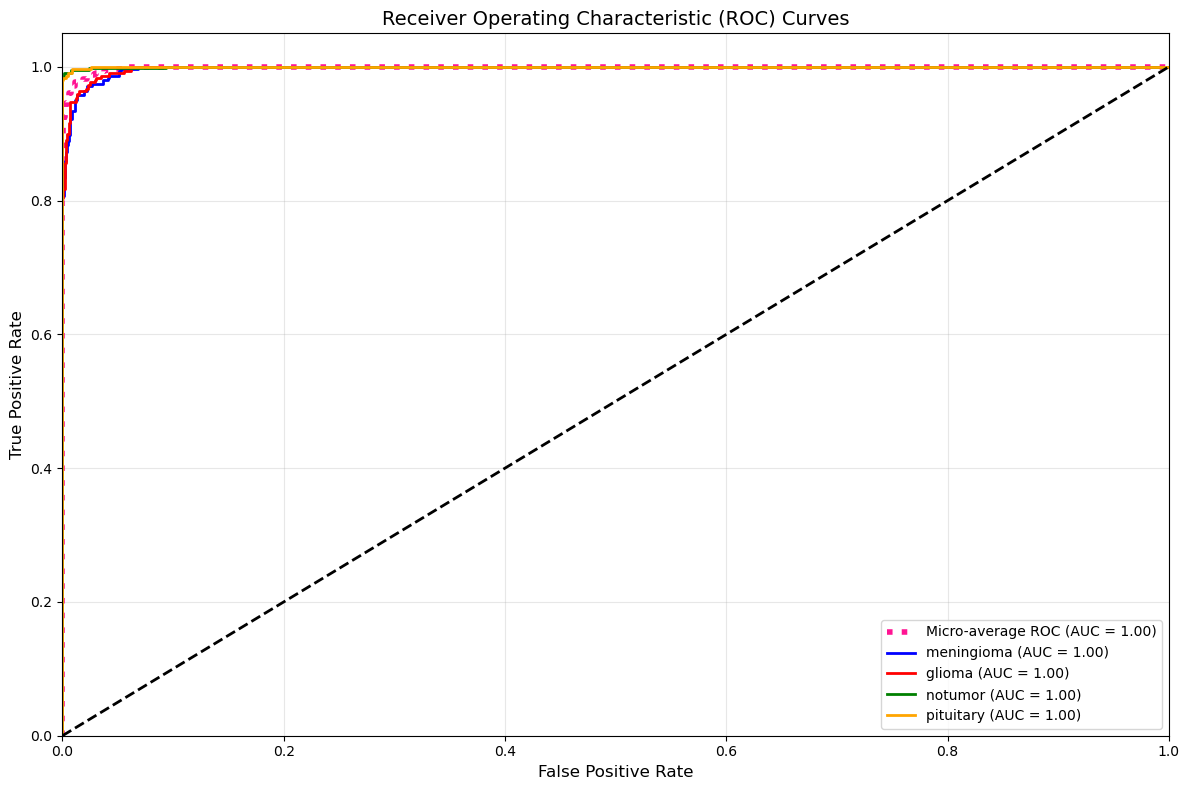
\includegraphics[width=0.9\linewidth]{Images/Metrices/roc.png}
    \caption{ROC Curve for Brain Tumor Classification Model}
    \label{fig:VGG16 ROC Curve}
\end{figure}

Our model achieved an AUC of 1.0 for all individual classes (meningioma,
glioma, notumor, pituitary) and for the micro-average. This indicates that the
model is able to distinguish between the different classes with almost perfect
accuracy based on this metric. The curves are all hugging the top-left corner
of the graph, which is the optimal position. The dashed black line represents a
random classifier (AUC = 0.5).

\item \textbf{Precision, Recall, and F1-score}
\begin{figure}[H]
    \centering
    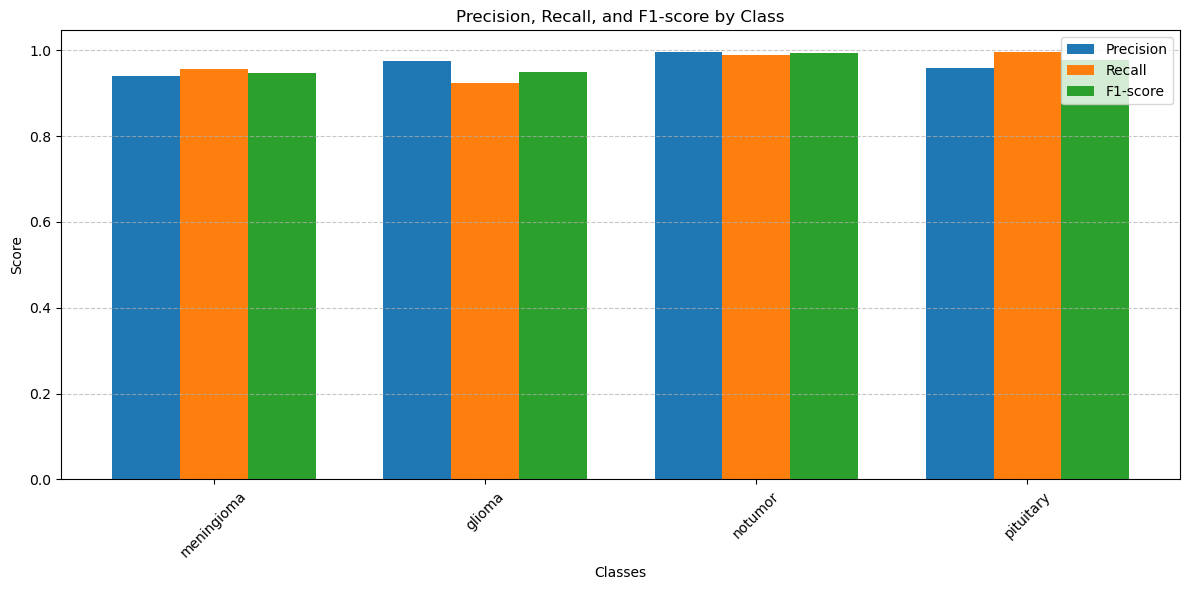
\includegraphics[width=1\linewidth]{Images/Metrices/scores.png}
    \caption{F1 Score, Precision, and Recall for VGG16 Model}
    \label{fig:VGG16 Scores}
\end{figure}

\begin{enumerate}
    \item \textbf{Precision}: Our model has high precision for all classes (above 0.95 for most), with "notumor" and "pituitary" being particularly high, indicating very few false positives.
    \item \textbf{Recall}: Our model also shows high recall across all classes, particularly for "notumor" and "pituitary," indicating it correctly identifies almost all instances of these classes.
    \item \textbf{F1-score}: The F1-scores are also very high (close to 0.98 for all classes), confirming the model's balanced performance in identifying classes correctly and comprehensively.
\end{enumerate}

\item \textbf{Model Training History}

\begin{figure}[H]
    \centering
    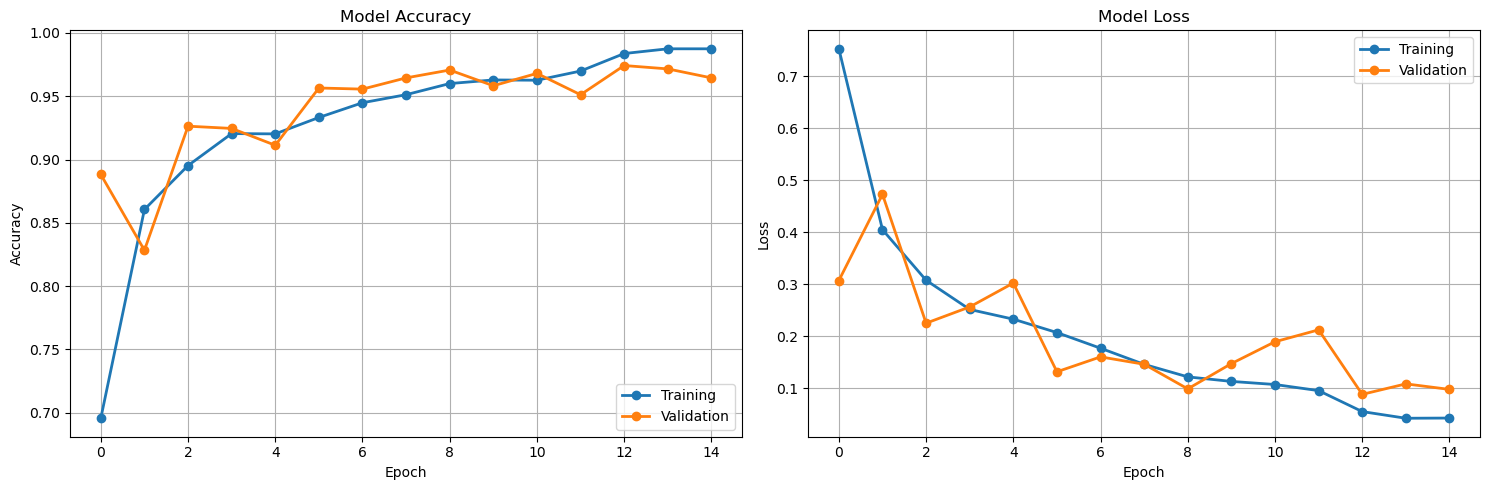
\includegraphics[width=1\linewidth]{Images/Metrices/traininghistory.png}
    \caption{Model Training History}
    \label{fig:Model Training History}
\end{figure}

This image shows the model's performance during the training process over 14 epochs.

\textbf{Model Accuracy:} The left plot shows both training accuracy (blue line) and validation accuracy (orange line). 
\begin{enumerate}[label=$\bullet$] 
    \item The training accuracy steadily increases and reaches a high of about 99\% by the final epoch.
    \item The validation accuracy also increases and closely follows the training accuracy, reaching a high of over 96\%.
    \item The closeness between the training and validation accuracy curves indicates that the model is learning effectively and generalizing well to new, unseen data, with no significant signs of overfitting.
\end{enumerate}

\textbf{Model Loss:} The right plot shows the training loss and validation loss.  
\begin{enumerate}[label=$\bullet$] 
    \item The training loss (blue line) decreases consistently throughout training, indicating the model is getting better at making correct predictions.
    \item The validation loss (orange line) also decreases, mirroring the training loss trend, which again suggests the model isn't overfitting. The validation loss shows some minor fluctuations, but the overall trend is a consistent decline.
\end{enumerate}

\item \textbf{Confusion Matrix}

\begin{figure}[H]
    \centering
    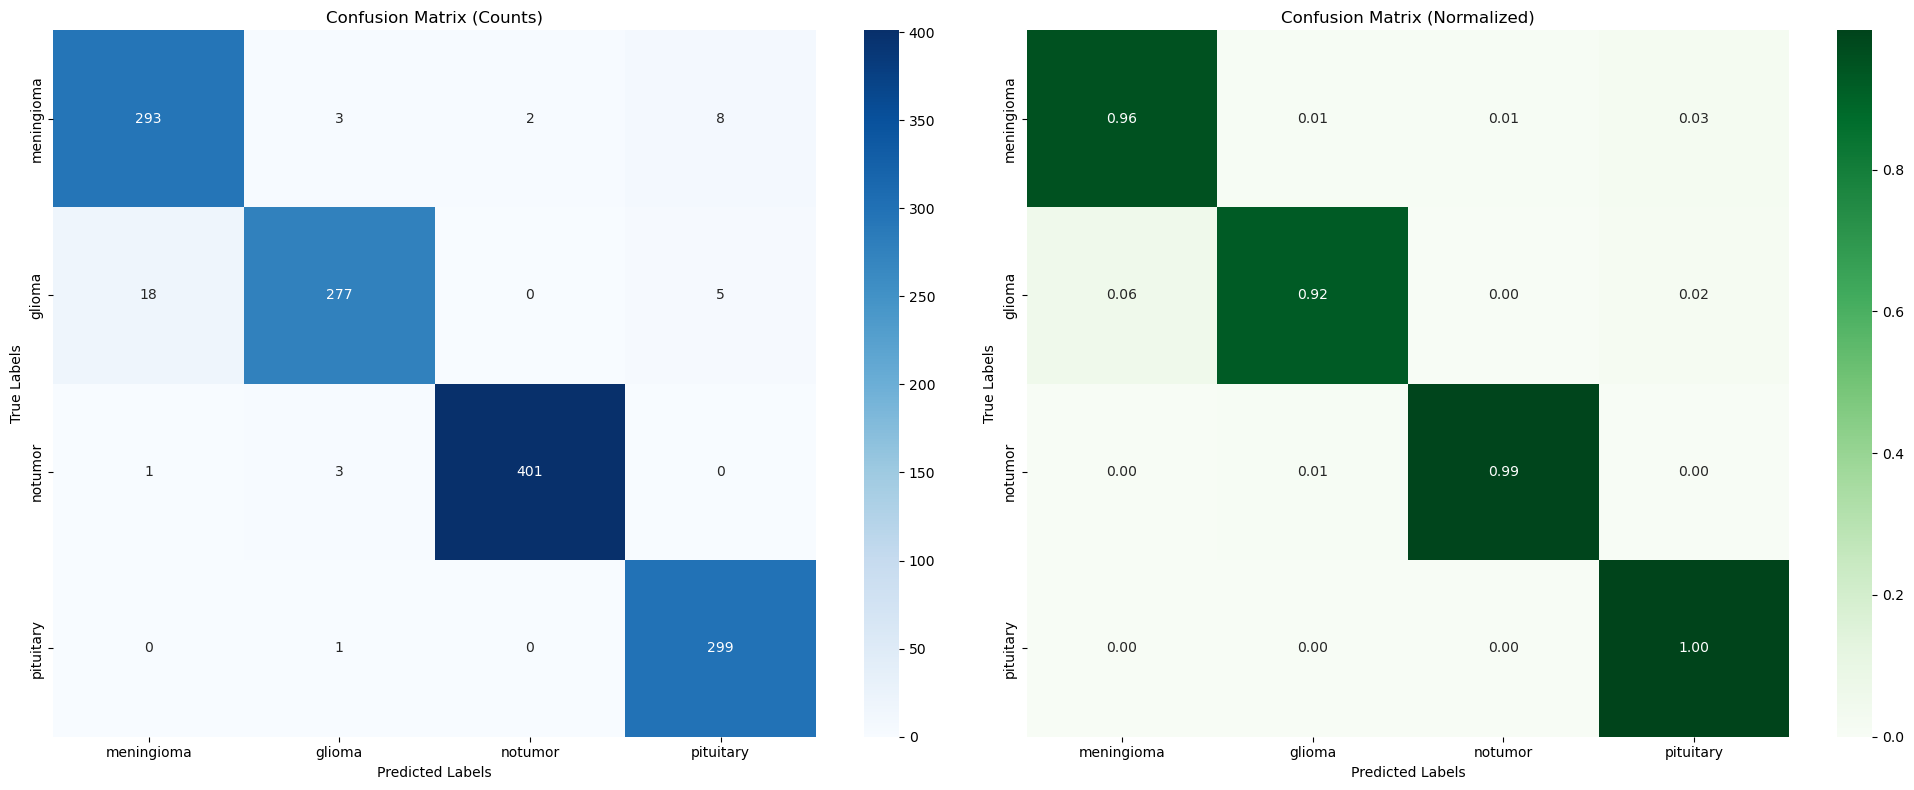
\includegraphics[width=1\linewidth]{Images/Metrices/confusion.png}
    \caption{Confusion Matrix for VGG16 Model}
    \label{fig:Confusion Matrix}
\end{figure}

The two heatmaps show the same data: the left one shows raw counts, and the right one shows normalized percentages.
\begin{enumerate}[label=$\bullet$] 

\item \textbf{Rows:} Represent the true labels (the actual class of the MRI).  

\item \textbf{Columns:} Represent the predicted labels (the class the model assigned).

\item \textbf{Diagonal Elements:} The numbers along the main diagonal (e.g., 293 for meningioma, 277 for glioma) represent the number of correct predictions for each class.

\item \textbf{Off-Diagonal Elements:} The numbers off the diagonal represent misclassifications.
\end{enumerate}

\textbf{Count Matrix (Left):} 
\begin{table}[h!]
\centering
\caption{Confusion matrix showing counts of correctly classified and misclassified MRI samples.}

\begin{tabular}{ccccc}
\toprule
\textbf{True Class} & \textbf{Meningioma} & \textbf{Glioma} & \textbf{Notumor} & \textbf{Pituitary} \\
\midrule
Meningioma & 293 & 3 & 2 & 8 \\
Glioma     & 18  & 277 & 0 & 5 \\
Notumor    & 0   & 0 & 401 & 0 \\
Pituitary  & 0   & 1 & 0 & 299 \\
\bottomrule
\end{tabular}
\end{table} 
% \begin{enumerate}[label=$\bullet$]
%     \item \textbf{Meningioma:} 293 were correctly classified, but 3 were mistaken for glioma, 2 for notumor, and 8 for pituitary.
%     \item \textbf{Glioma:} 277 were correct, but 18 were mistaken for meningioma, and 5 for pituitary.
%     \item \textbf{Notumor:} 401 were correct, with only a few misclassified.
%     \item \textbf{Pituitary:} 299 were correct, with only 1 misclassified as glioma.
% \end{enumerate}

\item \textbf{Normalized Matrix (Right):}  
\begin{enumerate}[label=$\bullet$]

\item This heatmap shows the same data as percentages of the total for each true class. 

\item The highest misclassification rate appears to be glioma being misclassified as meningioma (6\%), and meningioma being misclassified as pituitary (3\%). These are minor errors given the overall high accuracy.
\end{enumerate}
\end{enumerate}




